\section{Bits}

Section \secref{sec:arch:int} discussed the representation of integral numbers
and their associated operations as implemented by a computer processor.  This
section looks at numbers purely as (binary) data, with little or no arithmetic
interpretation given to their content.  Even so, just as it did for arithmetic
operations, the binary representation has unique characteristics that can be
used in the construction of algorithms and data structures.

In general, a collection of bits used in this way is called a \textit{bit set}.
The value of the set, interpreted as a signed or unsigned integer, is usually
irrelevant (except when fortuitously exploiting arithmetic hardware to implement
other operations, as will be shown).  Each bit in the set is said to be either
\textit{clear} or (sometimes confusingly) \textit{set}, depending on whether its
value is \texttt{0} or \texttt{1}, respectively.

\subsection{Mixed arithmetic/bitwise expressions}

\label{subsubsec:arch:mixed}

The properties of bitwise and arithmetic operations and the circuits that
implement them can be taken advantage of to build expressions that perform
interesting and useful computations.

\paragraph{\texttt{blsr}}

Listing \ref{lst:arch:blsr} shows how a combination of a subtraction (v.
\secrefpar{subsubsec:arch:sub}) and a bitwise \texttt{and} operation can be used
to clear the least-significant set bit in a number.  Listing
\ref{lst:arch:blsr_ops} demonstrates how the calculation works: subtracting one
results in a borrow in all trailing zeroes, ultimately borrowing from the
least-significant set bit.  As a result, this bit becomes a zero, while all
trailing zeroes become ones.  The resulting a bit mask, when combined with the
original values with an \texttt{and} operation, preserves all of the digits
except for the least-significant one, which is cleared.  In particular:

\begin{itemize}
    \item
        More-significant digits are preserved in the mask, so they remain the
        same after the operation (\texttt{1 \& 1 = 1}, \texttt{0 \& 0 = 0}).
    \item
        Less-significant digits all become one in the mask, so they are
        preserved.  This is irrelevant in this case, since they are known to be
        zero.
    \item
        The least-significant set bit is cleared, since the borrowing from the
        subtraction causes its position to become a zero in the mask.
\end{itemize}

\begin{figure}[ht]
    \centering
    \vspace{-\baselineskip}
    \begin{subfigure}[t]{0.45\textwidth}
        \begin{lstlisting}[
            style=c++,
            label={lst:arch:blsr},
            caption={\texttt{blsr} using subtraction},
        ]
template<std::unsigned_integral T>
constexpr auto blsr(T n) {
    return n & (n - T{1});
}
        \end{lstlisting}
    \end{subfigure}
    \begin{subfigure}[t]{0.45\textwidth}
        \begin{lstlisting}[
            label={lst:arch:blsr_ops},
            caption={\texttt{blsr} operations in detail},
            xleftmargin=4em,
        ]
 0b1100 = 12       0b1100 = 12
-0b0001 =  1  .-> &0b1011 = 11
-------       |   -------
 0b1011 = 11 -'    0b1000 =  8
        \end{lstlisting}
    \end{subfigure}
    \vspace{-\baselineskip}
\end{figure}

The function is named after the instruction in the x86 architecture which
performs the same operation.  It can in turn be used, for example, to check if a
number is a power of two --- i.e. if it has a single bit set (listing
\ref{lst:arch:is_pow2}).

\begin{figure}[ht]
    \vspace{-\baselineskip}
    \begin{lstlisting}[
        style=c++,
        label={lst:arch:is_pow2},
        caption={\texttt{is\_pow2} using \texttt{blsr}},
    ]
constexpr bool is_pow2(std::unsigned_integral auto n) {
    return n && !blsr(n);
}
    \end{lstlisting}
    \vspace{-2\baselineskip}
\end{figure}

\subsubsection{\texttt{tzcnt}}

Listing \ref{lst:arch:tzcnt} shows a method to count the trailing (i.e.
least-significant) consecutive zeroes in a binary number.  Listing
\ref{lst:arch:tzcnt_ops} demonstrates how the calculation works: it is
comparable to the one in the \texttt{blsr} example.  Negation of a number using
the two's complement representation (v. section
\secrefpar{sec:arch:ones_twos_comp}) is equivalent to the one's complement plus
one.  An \texttt{or} operation with the complement of the original value would
result in all bits being set; adding one prior to it causes all trailing ones to
revert to their original zero value and carry until the least-significant set
bit, which similarly reverts to a zero.  The resulting value is equal to the
complement, except all original trailing zeroes remain zeroes.  When the
\texttt{or} operation is performed, the result will have ones except in that
same original range of zeroes.  At this point, either complementing the result
and doing a population count or subtracting the population count from the total
number of bits will result in the number of trailing zeroes in the original
value.

\begin{figure}[ht]
    \centering
    \vspace{-\baselineskip}
    \begin{subfigure}[t]{0.5\textwidth}
        \lstinputlisting[
            style=c++,
            firstline=36,
            lastline=40,
            label={lst:arch:tzcnt},
            caption={\texttt{tzcnt}},
        ]{arch/bit/bit.cpp}
    \end{subfigure}
    \hspace{4em}
    \begin{subfigure}[t]{0.375\textwidth}
        \begin{lstlisting}[
            style=x86,
            label={lst:arch:tzcnt_ops},
            caption={\texttt{tzcnt} operations in detail},
        ]
 0b0010 n        0b0010 n
^0b1111     .-> |0b1110
-------     |   -------
 0b1101 ~n  |    0b1110 n | -n
+0b0001     |   ^0b1111
-------     |   -------
 0b1110 -n -'    0b0001

    popcount(0b0001) = 1
4 - popcount(0b1110) = 1
        \end{lstlisting}
    \end{subfigure}
    \vspace{-2\baselineskip}
\end{figure}

\subsection{Population count}

\label{subsec:arch:popcnt}

Counting the bits in a set which have the value \texttt{1} --- i.e.  its
\textit{population count} --- is a useful operation, since such
\textit{horizontal sum} can be used as the basis for other operations.  In the
simplest case, this sum is the number of elements present in the
set\footnotemark.

\footnotetext{
    Counting the bits which are \emph{not} set is essentially the same problem,
    and can be implemented based on the population count by either subtracting
    the result from the set size or by using the complement of the set as an
    input.
}

\paragraph{Linear}

A trivial implementation (listing \ref{lst:arch:popcnt_lin}) checks every digit
in the input and counts those that are set.  The code in the example examines
the least-significant bit of the input value on each iteration while
progressively shifting that value to the right.  This is done a number of times
equal to the number of binary digits in the input type \texttt{T}, so that all
digits are examined.

\footnotetext{
    Machine code in these examples shows the instantiation of the template
    functions for the \ident{std::uint32_t} type.
}

\begin{figure}[ht]
    \vspace{-\baselineskip}
    \begin{subfigure}[t]{0.65\textwidth}
        \lstinputlisting[
            style=c++,
            firstline=15,
            lastline=22,
            label={lst:arch:popcnt_lin},
            caption={Linear \texttt{popcnt}},
        ]{arch/bit/popcnt.cpp}
    \end{subfigure}
    \hspace*{\fill}
    \begin{subfigure}[t]{0.3\textwidth}
        \begin{lstlisting}[style=x86]
00: mov eax, 0x20
05: xor edx, edx
07: nop
10: mov ecx, edi
12: and ecx, 0x1
15: add edx, ecx
17: shr edi, 1
19: dec eax
1b: jne 10
1d: mov eax, edx
1f: ret
        \end{lstlisting}
    \end{subfigure}
    \vspace{-2\baselineskip}
\end{figure}

\paragraph{Shift}

Because testing whether a value (either in a register or the result of a
calculation) is zero is usually a primitive operation, the number of iterations
in the previous example can be reduced by terminating the loop when that
condition is detected --- i.e.  when there are no more set bits in the input.
This ignores higher-order bits in the input which are not set (listing
\ref{lst:arch:popcnt_shift}) and also removes the need for a separate counter.

\begin{figure}[ht]
    \vspace{-\baselineskip}
    \begin{subfigure}[t]{0.65\textwidth}
        \lstinputlisting[
            style=c++,
            firstline=28,
            lastline=34,
            label={lst:arch:popcnt_shift},
            caption={\texttt{popcnt} using bitwise shift},
        ]{arch/bit/popcnt.cpp}
    \end{subfigure}
    \hspace*{\fill}
    \begin{subfigure}[t]{0.3\textwidth}
        \begin{lstlisting}[style=x86]
00: xor  eax, eax
02: test edi, edi
04: je   20
06: nop
10: mov  edx, edi
12: and  edx, 0x1
15: add  eax, edx
17: shr  edi, 1
19: jne  10
1b: ret
1c: nop
20: ret
        \end{lstlisting}
    \end{subfigure}
    \vspace{-2\baselineskip}
\end{figure}

\paragraph{\texttt{blsr}}

Another operation which may be primitive is clearing the least significant bit.
Even if it is not, it can be implemented easily using other basic operations (v.
section \secrefpar{subsubsec:arch:mixed}).  Using this operation, the number of
iterations can be reduced to the number of set bits in the input (listing
\ref{lst:arch:popcnt_blsr}).  Compared to the more advanced methods below, this
can be more efficient if the number of set bits is known to be
small\footnotemark.

\footnotetext{
    I.e. if the population count is known to be low (or high, since
    complementing the input and subtracting the result from the total number of
    bits are simple operations).
}

\begin{figure}[ht]
    \vspace{-\baselineskip}
    \begin{subfigure}[t]{0.65\textwidth}
        \lstinputlisting[
            style=c++,
            firstline=45,
            lastline=51,
            label={lst:arch:popcnt_blsr},
            caption={\texttt{popcnt} using \texttt{blsr}},
        ]{arch/bit/popcnt.cpp}
    \end{subfigure}
    \hspace*{\fill}
    \begin{subfigure}[t]{0.3\textwidth}
        \begin{lstlisting}[style=x86]
00: xor  eax, eax
02: test edi, edi
04: je   20
06: nop
10: inc  eax
12: blsr edi, edi
17: jne  10
19: ret
1a: nop
20: ret
        \end{lstlisting}
    \end{subfigure}
    \vspace{-2\baselineskip}
\end{figure}

\paragraph{Instruction}

Of course, most processors have a dedicated instruction for this operation, and
the C++ 20 standard library includes a version which is likely to generate it
directly when available (listing \ref{lst:arch:popcnt_instr}).

\begin{figure}[ht]
    \centering
    \vspace{-\baselineskip}
    \begin{subfigure}[t]{0.65\textwidth}
        \lstinputlisting[
            style=c++,
            firstline=57,
            lastline=60,
            label={lst:arch:popcnt_instr},
            caption={\texttt{popcnt} instruction},
        ]{arch/bit/popcnt.cpp}
    \end{subfigure}
    \hspace*{\fill}
    \begin{subfigure}[t]{0.3\textwidth}
        \begin{lstlisting}[style=x86]
00: xor    eax, eax
02: popcnt eax, edi
06: ret
        \end{lstlisting}
    \end{subfigure}
    \vspace{-2\baselineskip}
\end{figure}

\paragraph{Table}

Another approach is to precompute the counts for all possible byte values and
simply consult them at runtime (listing \ref{lst:arch:popcnt_table}).  This
requires 256 bytes of storage in machines with 8-bit bytes.  Whether it is
advantageous depends on whether the resulting memory accesses are faster than
performing the computation.

\begin{figure}[ht]
    \centering
    \vspace{-\baselineskip}
    \begin{subfigure}[t]{0.55\textwidth}
        \lstinputlisting[
            style=c++,
            firstline=66,
            lastline=83,
            label={lst:arch:popcnt_table},
            caption={\texttt{popcnt} using a table},
        ]{arch/bit/popcnt.cpp}
    \end{subfigure}
    \hspace*{\fill}
    \begin{subfigure}[t]{0.4\textwidth}
        \begin{lstlisting}[style=x86]
lea   rcx, [rip+0xd99]
mov   edx, edi
movzx eax, dil
mov   eax, DWORD PTR [rcx+rax*4]
movzx esi, dh
mov   esi, esi
add   eax, DWORD PTR [rcx+rsi*4]
mov   esi, edi
shr   esi, 0x10
movzx esi, sil
add   eax, DWORD PTR [rcx+rsi*4]
shr   edx, 0x18
add   eax, DWORD PTR [rcx+rdx*4]
ret
        \end{lstlisting}
    \end{subfigure}
    \vspace{-2\baselineskip}
\end{figure}

\paragraph{Sums}

One interesting method of computing the population count is the following sum,
where $n$ is the number of bits in $x$:
\begin{align*}
    \texttt{popcnt}(x)
        &= x - \sum_{i=1}^{n-1} \left\lfloor 2^{-i}x \right\rfloor
        \\[0.5\baselineskip]
        &= x
            - \left\lfloor \frac{x}{2}       \right\rfloor
            - \left\lfloor \frac{x}{4}       \right\rfloor
            - \left\lfloor \frac{x}{8}       \right\rfloor
            - \ldots
            - \left\lfloor \frac{x}{2^{n-1}} \right\rfloor
\end{align*}

This equality can be demonstrated to be correct by decomposing each term as a
binary number followed by some elementary algebra\footnotemark.  E.g. for a
4-bit number, where $b_n$ is the $n\text{th}$ least-significant bit of $x$:
\begin{align*}
    \texttt{popcnt}(x)
        &= x
            - \left\lfloor \frac{x}{2} \right\rfloor
            - \left\lfloor \frac{x}{4} \right\rfloor
            - \left\lfloor \frac{x}{8} \right\rfloor \\
        &= (2^3b_3+2^2b_2+2^1b_1+2^0b_0)
            - (2^2b_3+2^1b_2+2^0b_1)
            - (2^1b_3+2^0b_2)
            - (2^0b_3) \\
        &= b_3(2^3-2^2-2^1-2^0) + b_2(2^2-2^1-2^0) + b_1(2^1-2^0) + b_0(2^0) \\
        &= b_3(1) + b_2(1) + b_1(1) + b_0(1) \\
        &= b_3 + b_2 + b_1 + b_0
\end{align*}

\footnotetext{
    It may also be helpful to think of the divisions by powers of 2 as
    right-shift operations on a binary number.
}

It is, however, not very practical from a computational perspective when
compared to the other methods shown here since it requires $n - 1$ shifts and
subtractions.  Still, it makes for very simple and compact code (listing
\ref{lst:arch:popcnt_sum}) and can be partially used in other methods.

\begin{figure}[ht]
    \vspace{-\baselineskip}
    \begin{subfigure}[t]{0.65\textwidth}
        \lstinputlisting[
            style=c++,
            firstline=89,
            lastline=94,
            label={lst:arch:popcnt_sum},
            caption={\texttt{popcnt} as a sum},
        ]{arch/bit/popcnt.cpp}
    \end{subfigure}
    \hspace*{\fill}
    \begin{subfigure}[t]{0.3\textwidth}
        \begin{lstlisting}[style=x86]
00: mov edx, edi
02: shr edx, 1
04: mov eax, edi
06: je  16
08: nop
10: sub eax, edx
12: shr edx, 1
14: jne 10
16: ret
        \end{lstlisting}
    \end{subfigure}
    \vspace{-\baselineskip}
\end{figure}

Another interesting sum is the following (listing \ref{lst:arch:popcnt_rot}):
\begin{align*}
    \texttt{popcnt}(x)
        &= -\sum_{i=0}^{n-1} (x ~ \overset{rot}{\texttt{<{}<}} ~ i)
\end{align*}

Where $n$ is again the number of bits in $x$, the $\overset{rot}{\texttt{<{}<}}$
operation is a circular left shift (the direction is irrelevant, right shift
could equally be used), and the summation is done modulo $2^n$.  The final
negation must be done in two's complement representation.  Demonstrated again
with a 4-bit number:
\begin{alignat*}{3}
    \texttt{popcnt}(x)
        &= && ~ -(x
            + x ~ \overset{rot}{\texttt{<{}<}} ~ 1
            + x ~ \overset{rot}{\texttt{<{}<}} ~ 2
            + x ~ \overset{rot}{\texttt{<{}<}} ~ 3
        ) \\
        &= && ~ -(2^3b_3+2^2b_2+2^1b_1+2^0b_0 \\
        &  && \quad +2^2b_3+2^1b_2+2^0b_1+2^3b_0 \\
        &  && \quad +2^1b_3+2^0b_2+2^3b_1+2^2b_0 \\
        &  && \quad +2^0b_3+2^3b_2+2^2b_1+2^1b_0) \\
        &= && ~ -(2^3+2^2+2^1+2^0)(b_3+b_2+b_1+b_0) \\
        &= && ~ -(2^4-1)(b_3+b_2+b_1+b_0) \\
        &= && ~ -(2^4(b_3+b_2+b_1+b_0) - (b_3+b_2+b_1+b_0)) \\
        &= && ~ -2^4(b_3+b_2+b_1+b_0) + (b_3+b_2+b_1+b_0) \\
        &\equiv&&_{\bmod 2^4} ~ b_3+b_2+b_1+b_0
\end{alignat*}

\begin{figure}[ht]
    \centering
    \vspace{-\baselineskip}
    \begin{subfigure}[t]{0.65\textwidth}
        \lstinputlisting[
            style=c++,
            firstline=100,
            lastline=107,
            label={lst:arch:popcnt_rot},
            caption={\texttt{popcnt} using circular shift},
        ]{arch/bit/popcnt.cpp}
    \end{subfigure}
    \hspace*{\fill}
    \begin{subfigure}[t]{0.3\textwidth}
        \begin{lstlisting}[style=x86]
00: mov  edx, 0x20
05: xor  eax, eax
07: nop
10: add  eax, edi
12: rorx edi, edi, 0x1f
18: dec  edx
1a: jne  00
1c: neg  eax
1e: ret
        \end{lstlisting}
    \end{subfigure}
    \vspace{-2\baselineskip}
\end{figure}

\paragraph{Binary division}

Yet another approach is to use a very common strategy in computing: reducing the
problem size by half on each iteration.  The count of a 32-bit number is the sum
of each of its 16-bit halves, which in turn is the sum of each of its halves,
and so on recursively until groups of single bits are examined.  The count for a
single bit is obviously the bit itself, establishing the base case of the
recursive process.  This calculates the population count in a number of steps
proportional to the binary logarithm of the number of bits.  The diagram below
shows this process for an 8-bit number.

\begin{center}
    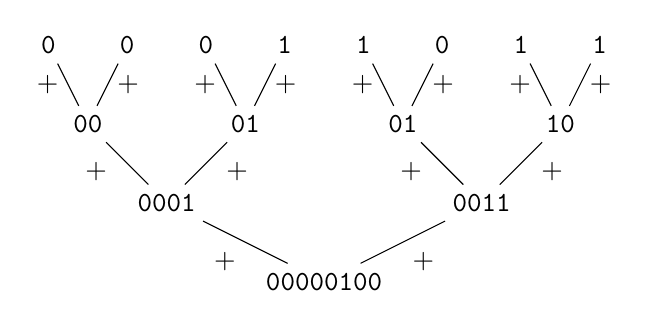
\begin{tikzpicture}[xscale = 0.5, font = \ttfamily]
        \node (n00) at ( 0, 3) {0};
        \node (n01) at ( 2, 3) {0};
        \node (n02) at ( 4, 3) {0};
        \node (n03) at ( 6, 3) {1};
        \node (n04) at ( 8, 3) {1};
        \node (n05) at (10, 3) {0};
        \node (n06) at (12, 3) {1};
        \node (n07) at (14, 3) {1};
        \node (n10) at ( 1, 2) {00};
        \node (n11) at ( 5, 2) {01};
        \node (n12) at ( 9, 2) {01};
        \node (n13) at (13, 2) {10};
        \node (n20) at ( 3, 1) {0001};
        \node (n21) at (11, 1) {0011};
        \node (n30) at ( 7, 0) {00000100};
        \draw (n00) -- node [pos = 0.50, anchor = east] {$+$} (n10);
        \draw (n01) -- node [pos = 0.50, anchor = west] {$+$} (n10);
        \draw (n02) -- node [pos = 0.50, anchor = east] {$+$} (n11);
        \draw (n03) -- node [pos = 0.50, anchor = west] {$+$} (n11);
        \draw (n04) -- node [pos = 0.50, anchor = east] {$+$} (n12);
        \draw (n05) -- node [pos = 0.50, anchor = west] {$+$} (n12);
        \draw (n06) -- node [pos = 0.50, anchor = east] {$+$} (n13);
        \draw (n07) -- node [pos = 0.50, anchor = west] {$+$} (n13);
        \draw (n10) -- node [pos = 0.25, anchor = north east] {$+$} (n20);
        \draw (n11) -- node [pos = 0.25, anchor = north west] {$+$} (n20);
        \draw (n12) -- node [pos = 0.25, anchor = north east] {$+$} (n21);
        \draw (n13) -- node [pos = 0.25, anchor = north west] {$+$} (n21);
        \draw (n20) -- node [pos = 0.50, anchor = north east] {$+$} (n30);
        \draw (n21) -- node [pos = 0.50, anchor = north west] {$+$} (n30);
    \end{tikzpicture}
\end{center}

Listing \ref{lst:arch:popcnt_bin} shows a very efficient implementation.  It
uses a technique known as \textit{SIMD Within A Register} (SWAR), meaning a
single register is treated as several groups of data and each calculation is
done for all of those groups in a single instruction.  This implementation is
very generic and works for types of any width.  Figure \ref{fig:arch:popcnt_bin}
shows the masks and shift operations involved in each step for an 8-bit number.

\begin{figure}[ht]
    \vspace{-\baselineskip}
    \begin{subfigure}[t]{0.7\textwidth}
        \lstinputlisting[
            style=c++,
            firstline=113,
            lastline=133,
            label={lst:arch:popcnt_bin},
            caption={$\log_2$ \texttt{popcnt}},
        ]{arch/bit/popcnt.cpp}
    \end{subfigure}
    \begin{subfigure}[t]{0.275\textwidth}
        \begin{lstlisting}[style=x86]
mov   eax, edi
shr   edi, 1
and   eax, 0x55555555
and   edi, 0x55555555
add   eax, edi
mov   edx, eax
shr   edx, 0x2
and   eax, 0x33333333
and   edx, 0x33333333
add   edx, eax
mov   eax, edx
shr   eax, 0x4
and   edx, 0xf0f0f0f
and   eax, 0xf0f0f0f
add   eax, edx
mov   edx, eax
shr   edx, 0x8
and   eax, 0xff00ff
and   edx, 0xff00ff
add   edx, eax
movzx eax, dx
shr   edx, 0x10
add   eax, edx
ret
        \end{lstlisting}
    \end{subfigure}
    \vspace{-\baselineskip}
\end{figure}

\begin{figure}[p]
    \centering
    \begin{tikzpicture}[>={Stealth[round]}, font = \ttfamily]
    \node (n0) [draw] at (0, 0) {0 0 0 1 1 0 1 1};
    \node (shift0) [right = 1.5 of n0] {0 0 0 0 1 1 0 1};
    \node (and0_0) [draw, circle, below = 0.5 of n0] {\&};
    \node (and0_1) [draw, circle, below = 0.5 of shift0] {\&};
    \node (mask0) [right = 0.45 of and0_0] {0 1 0 1 0 1 0 1};
    \node (n0_0) [below = 0.5 of and0_0] {00 01 00 01};
    \node (n0_1) [below = 0.5 of and0_1] {00 00 01 01};
    \node (p0) [draw, circle, below = 0.5 of n0_0] {$+$};
    \node (n1) [draw, below = 0.5 of p0] {00 01 01 10};
    \node (shift1)
        at ($ (0, 0)!(shift0)!(1, 0) + (0, 0)!(n1)!(0, 1) $)
        {00 00 01 01};
    \node (and1_0) [draw, circle, below = 0.5 of n1] {\&};
    \node (and1_1) [draw, circle, below = 0.5 of shift1] {\&};
    \node (mask1)
        at ($ (0, 0)!(mask0)!(1, 0) + (0, 0)!(and1_0)!(0, 1) $)
        {00 11 00 11};
    \node (n1_0) [below = 0.5 of and1_0] {0001 0010};
    \node (n1_1) [below = 0.5 of and1_1] {0000 0001};
    \node (p1) [draw, circle, below = 0.5 of n1_0] {$+$};
    \node (n2) [draw, below = 0.5 of p1] {0001 0011};
    \node (shift2)
        at ($ (0, 0)!(shift0)!(1, 0) + (0, 0)!(n2)!(0, 1) $)
        {0000 0001};
    \node (and2_0) [draw, circle, below = 0.5 of n2)] {\&};
    \node (and2_1) [draw, circle, below = 0.5 of shift2)] {\&};
    \node (mask2)
        at ($ (0, 0)!(mask0)!(1, 0) + (0, 0)!(and2_0)!(0, 1) $)
        {0000 1111};
    \node (n2_0) [below = 0.5 of and2_0] {00000011};
    \node (n2_1) [below = 0.5 of and2_1] {00000001};
    \node (p2) [draw, circle, below = 0.5 of n2_0] {$+$};
    \node (s) [draw, below = 0.5 of p2] {00000100};
    \draw[->] ($ (n0) + (0, 1) $) -- (n0);
    \draw[->] (n0) -- node [pos = 0.5, anchor = south] {>{}>1} (shift0);
    \draw (n0) -- (and0_0);
    \draw (shift0) -- (and0_1);
    \draw (mask0) -- (and0_0);
    \draw (mask0) -- (and0_1);
    \draw[->] (and0_0) -- (n0_0);
    \draw[->] (and0_1) -- (n0_1);
    \draw (n0_0) -- (p0);
    \draw (n0_1) |- (p0);
    \draw[->] (p0.south) -- +(0, -0.25) -| (n1.north);
    \draw (n1) -- (and1_0);
    \draw (shift1) -- (and1_1);
    \draw (mask1) -- (and1_0);
    \draw (mask1) -- (and1_1);
    \draw[->] (and1_0) -- (n1_0);
    \draw[->] (and1_1) -- (n1_1);
    \draw[->] (n1) -- node [pos = 0.5, anchor = south] {>{}>2} (shift1);
    \draw (n1_0) -- (p1);
    \draw (n1_1) |- (p1);
    \draw[->] (p1.south) -- +(0, -0.25) -| (n2.north);
    \draw[->] (n2) -- node [pos = 0.5, anchor = south] {>{}>4} (shift2);
    \draw (n2) -- (and2_0);
    \draw (shift2) -- (and2_1);
    \draw (mask2) -- (and2_0);
    \draw (mask2) -- (and2_1);
    \draw[->] (and2_0) -- (n2_0);
    \draw[->] (and2_1) -- (n2_1);
    \draw (n2_0) -- (p2);
    \draw (n2_1) |- (p2);
    \draw[->] (p2) -- (s);
\end{tikzpicture}

    \caption{$\log_2$ \texttt{popcnt} for an 8-bit number}
    \label{fig:arch:popcnt_bin}
\end{figure}

\paragraph{CSA}

Performing a population count of several integer values can be a simple matter
of adding the counts of each, but a more efficient method is to use a Carry-Save
Adder (CSA).  This is a circuit used to implement one-digit binary addition
(section \secrefpar{subsubsec:arch:add} shows similar circuits).  It takes three
bits as input (the two values and the previous carry) and has two bits as output
(the sum and the carry) --- it in effect compresses three bits into two.

\begin{wrapfigure}{r}{0.2\textwidth}
    \vspace{-2\baselineskip}
    \begin{lstlisting}[
        label={lst:arch:csa},
        caption={CSA},
    ]
 1111 0000 v0
 1100 1100 v1
+1010 1010 v2
 ---------
 1110 1000 carry
 1001 0110 sum
    \end{lstlisting}
\end{wrapfigure}

This can be used to operate on three values at a time --- one accumulator and
two of the input integers.  The CSA is used to combine bits in the same position
in each of the three inputs.  These circuits can be connected in many ways, and
some result in better performance for certain types of inputs.  Listing
\ref{lst:arch:popcnt_csa} shows a simple implementation.

\begin{figure}[ht]
    \vspace{-\baselineskip}
    \lstinputlisting[
        style=c++,
        firstline=139,
        lastline=157,
        label={lst:arch:popcnt_csa},
        caption={\texttt{popcnt} using a CSA},
    ]{arch/bit/popcnt.cpp}
    \vspace{-\baselineskip}
\end{figure}

\subsection{Binary mask}

One very useful construct when dealing with binary data is the \textit{binary
mask}.  This mask is very similar to a \textit{boolean} value in that it has
only two possible values, but instead of representing the \texttt{true} value as
\texttt{1}, a value where all bits are set to \texttt{1} is used instead.  For
example, for a 4-bit binary number:

\begin{center}
    \begin{tabular}{l|cc}
        & \texttt{bool} & mask \\
        \hline
        \texttt{true}  & \texttt{0001} & \texttt{1111} \\
        \texttt{false} & \texttt{0000} & \texttt{0000} \\
    \end{tabular}
\end{center}

This type of mask is used extensively in programs which do logical and numeric
extensively, since they can be combined with other operations to very
efficiently implement branch-less conditionals, selections, etc.  While boolean
results in languages such as C yield the traditional \texttt{bool} values, whose
stored value is dictated to be either \texttt{0} or \texttt{1}, converting
between these two representations can be done very simply and
efficiently\footnotemark:

\footnotetext{
    \ident{to\_bool} could equally be implemented as \texttt{m \& 1}, which
    would generate an \texttt{and} instruction.  The implementation shown here
    is simpler and generalizes to more than pure binary masks, but both can be
    useful depending on the context.
}

\begin{multicols}{2}
    \begin{lstlisting}[style=c]
bool to_bool(u32 m) {
    return m;
}

u32 to_mask(bool b) {
    return -b;
}
    \end{lstlisting}
    \columnbreak
    \begin{lstlisting}[style=x86]
to_bool:
    test  edi, edi
    setne al
    ret
to_mask:
    movzx eax, dil
    neg   eax
    ret
    \end{lstlisting}
\end{multicols}
\vspace{-\baselineskip}

It should be noted that the generated code shown on the right gives an idea of
how these operations can be translated to machine code, but is very artificial.
Other than the additional requirements of the calling convention, there are a
variety of ways to generate both types of values from ALU operations.  The
actual code generated when these operations are combined with those preceding
and succeeding them will be highly variable, but will invariably be composed of
simple, elemental instructions.  In particular, very rarely will they generate a
combination of a conditional and jump instructions.  Compilers can generally
turn this sort of operations into very efficient code.  For example, if the
input is a regular integer, not a \texttt{bool}:

\begin{multicols}{2}
    \begin{lstlisting}[style=c]
u32 to_mask_u32(u32 x) {
    return to_mask(x);
}
    \end{lstlisting}
    \columnbreak
    \begin{lstlisting}[style=x86]
to_mask_u32:
    neg edi
    sbb eax, eax
    ret
    \end{lstlisting}
\end{multicols}

\subsection{From another bit}

This example (listing \ref{lst:arch:set_bit0}) shows a case where a binary mask
is advantageous.  It sets the value of a given bit in a byte based on the value
of another.  This might be used to change a flag in a bit set based on another.

\begin{figure}[ht]
    \centering
    \vspace{-\baselineskip}
    \begin{subfigure}[t]{0.5\textwidth}
        \lstinputlisting[
            style=c++,
            firstline=19,
            lastline=23,
            label={lst:arch:set_bit0},
            caption={Setting a bit based on another},
        ]{arch/bit/bit.cpp}
    \end{subfigure}
    \hspace{2em}
    \begin{subfigure}[t]{0.2\textwidth}
        \begin{lstlisting}[style=x86]
mov eax, edi
shr al, 4
and eax, 1
neg eax
xor eax, edi
and eax, 4
xor eax, edi
ret
        \end{lstlisting}
    \end{subfigure}
    \vspace{-\baselineskip}
\end{figure}

The binary mask allows the code to operate independently of the position of the
two bits.  In particular, they could be values provided at run time and a
similar sequence of operations could be used (listing \ref{lst:arch:set_bit1}).

\begin{figure}[ht]
    \centering
    \vspace{-\baselineskip}
    \begin{subfigure}[t]{0.5\textwidth}
        \lstinputlisting[
            style=c++,
            firstline=29,
            lastline=32,
            label={lst:arch:set_bit1},
            caption={Setting a bit based on another (param.)},
        ]{arch/bit/bit.cpp}
    \end{subfigure}
    \hspace{2em}
    \begin{subfigure}[t]{0.2\textwidth}
        \begin{lstlisting}[style=x86]
test  sil, dil
setne al
neg   eax
xor   eax, edi
and   eax, edx
xor   eax, edi
ret
        \end{lstlisting}
    \end{subfigure}
    \vspace{-\baselineskip}
\end{figure}

\subsection{Exercises}

\begin{enumerate}[label*=\arabic*.]
    \item
        \label{ex:arch:width_type}
        The return value of the \texttt{popcnt} function in listing
        \ref{lst:arch:blsr} is \texttt{int}.
        \begin{enumerate}[label*=\arabic*.]
            \item
                \label{ex:arch:width_type:range}
                Does that provide an acceptable range of values?  If not, what
                type would be most appropriate for the return value?  Would the
                answer be different if we wanted to optimize for calculation
                speed or data size?  What is the relationship between the type
                of the input and range of possible returned values?
            \item
                \label{ex:arch:width_type:impl}
                Write a type metafunction (v. section \secrefpar{sec:c++:meta})
                that returns the smallest type able to store the number of bits
                in an unsigned integer of a given type.
        \end{enumerate}
    \item
        \label{ex:arch:chess}
        Describe possible forms of storage for the state of the board in a game
        of chess and their advantages.
\end{enumerate}
